\newpage
\renewcommand{\arraystretch}{1.5}
\newcommand{\code}{\texttt}
\section{Datenbankentwurf}
\def \currentAuthor{Elias Gabl}

\subsection{Tabellenbeschreibung der Datenbank von OSTicket}

In dieser Dokumentation finden Sie eine grobe Beschreibung der Datenbank des Systems OS Ticket. OS Ticket ist ein Ticketsingsystem, das für einfache Support Anwendung entwickelt worden ist. Die Datenbank besteht aus 59 Tabellen, von diesen sind manche nicht mehr aktuell bzw. werden nicht mehr gebraucht, sind aber dennoch vorhanden. Daher werden in dieser Dokumentation nur die wichtigsten Tabellen der Datenbank beschrieben.\\
In gewissen Spalten ist es leider nicht möglich den Inhalt anzugeben, da es keine gute Dokumentation der Datenbank gibt und man den Inhalt der Spalten aus dem Kontext erschließen muss.
\newline
\newline
An dieser Stelle sollte ein Datenmodell stehen, aber da jenes von OSTicket recht groß und komplex ist, hat es hier nicht Platz. Sie finden es auf dem mitgelieferten Datenträger.(Der Dateiname ist: OSTicketDB.mwb).


\newpage

\subsubsection{ost\_config}

In dieser Tabelle werden wichtige Informationen über das System OSTicket gespeichert. Die Werte werden mit einem Schlüssel in der Datenbank abgelegt (Key und Value).
Diese Tabelle hat keine Referenz zu anderen Tabellen.

\begin{table}[h]
	\begin{tabular}{|p{3.5cm}|p{4cm}|p{6.2cm}|}
		\hline
		\textbf{Column Name:} & \textbf{Datatype:} & \textbf{Content:}\\
		\hline
		id & INT(11) & Eindeutg ID der Information. Dieser Wert ist rein technisch und hat neben der Eindeutigkeit keine weitere 
		Aussagekraft. \\
		\hline
		namespace & VARCHAR(64) & \\
		\hline
		key & VARCHAR(64) & Key der Information um die Suche zu erleichtern\\
		\hline
		value & TEXT & Informations Inhalt\\
		\hline
		updated & DATETIME & Erstelldatum der Information\\
		\hline
	\end{tabular}
	\caption{tab:ost-config}
\end{table}
\label{tab:ost_config}
\newpage


\subsubsection{ost\_attachment}

Sämtliche Informationen über den Anhang eines Tickets finden sich in dieser Tabelle. Beinhaltet sind der Datentyp, der Name, und die id des Anhanges. 

\begin{table}[h]
	\begin{tabular}{|p{3.5cm}|p{4cm}|p{6.2cm}|}
		\hline
		\textbf{Column Name:} & \textbf{Datatype:} & \textbf{Content:} \\
		\hline
		id & INT(10) & Eindeutige ID des Anhanges. Dieser Wert ist rein technisch und hat neben der Eindeutigkeit keine weitere  \\
		\hline
		object\_id & int(11) & Referenz auf ein Object das dem Anhang übergeben wird \\
		\hline
		type & CHAR(1) & Datentyp des Anhanges \\
		\hline
		file\_id & int(11) & Referenz auf das File das sich im Anhang befindet\\
		\hline
		name & VARCHAR(255) & Name des Anhanges \\
		\hline
		inline & TINYINT(1) & Beschreibt den Zitierstil des Anhangs \\
		\hline
		lang & VARCHAR(16) & Die Sprache in der, der Anhang verfasst wurde \\
		\hline
	\end{tabular}
	\caption{tab:ost-attachment}
\end{table}
\label{tab:ost_attachment}

\newpage

\subsubsection{ost\_canned\_response}

In dieser Tabelle werden vorgefertigte Antworten für Tickets abgelegt. Über die Antwort wird der Titel, die Sprache, der Inhalt, das Erstelldatum und das Änderungsdatum gespeichert.

\begin{table}[h]
	\begin{tabular}{|p{3.5cm}|p{4cm}|p{6.2cm}|}
		\hline
		\textbf{Column Name:} & \textbf{Datatype:} & \textbf{Content:}\\
		\hline
		canned\_id & INT(10) & Eindeutige ID der Nachricht. Dieser Wert ist rein technisch und hat neben der Eindeutigkeit keine weitere 
		Aussagekraft.\\
		\hline
		dept\_id & int(10) & Referenz auf die Abteilungen die diese Nachricht verwenden können\\
		\hline
		isenabled & TINYINT(1) & Gibt an ob die Nachricht freigegeben ist oder nicht.\\
		\hline
		titel & VARCHAR(255) & Titel der Nachricht\\
		\hline
		response & TEXT & Text den die Nachricht beinhaltet\\
		\hline
		lang & VARCHAR(16) & Sprache der Nachricht\\
		\hline
		notes & TEXT & Anmerkung zur Nachricht\\
		\hline
		created & DATETIME & Erstelldatum der Nachricht\\
		\hline
		updated & DATETIME & Änderungsdatum der Nachricht\\
		\hline
	\end{tabular}
	\caption{tab:ost-canned-response}
\end{table}
\label{tab:ost_canned_response}

\newpage

\subsubsection{ost\_content}

In dieser Tabelle werden Inhalte der Seiten aufgenommen. Es wird angeben, ob der Inhalt aktiv ist oder nicht. Jeder Inhalt umfasst auch einen Titel und einen Body. Zusätzlich werden noch der Typ und das Erstell- /Änderungsdatum angegeben.

\begin{table}[h]
	\begin{tabular}{|p{3.5cm}|p{4cm}|p{6.2cm}|}
		\hline
		\textbf{Column Name:} & \textbf{Datatype:} & \textbf{Content:}\\
		\hline
		id & INT(10) & Eindeutige ID des Contents. Dieser Wert ist rein technisch und hat neben der Eindeutigkeit keine weitere 
		Aussagekraft.\\
		\hline
		isactive & TINYINT(1) & Gib an ob der Inhalt aktiv ist oder nicht\\
		\hline
		type & VARCHAR(32) & Gib den Typ vom Inhalt an\\
		\hline
		name & VARCHAR(255) & Name vom Inhalt\\
		\hline
		body & TEXT & Der Bodyinhalt des Seiten Content\\
		\hline
		notes & TEXT & Anmerkungen zum Content\\
		\hline
		created & DATETIME & Erstelldatum des Content\\
		\hline
		updated & DATETIME & Änderungsdatum des Content\\
		\hline
	\end{tabular}
	\caption{tab:ost-content}
\end{table}
\label{tab:ost_content}

\newpage

\subsubsection{ost\_department}

Diese Tabelle speichert Informationen über eine Abteilung. Jede Abteilung hat einen Namen und eine Signatur. Ein Feld, das angibt, ob die Abteilung öffentlich ist oder nicht. Zudem wird festgehalten, zu welcher Gruppe die Abteilung gehört und wann diese erstellt worden ist.

\begin{table}[h]
	\begin{tabular}{|p{3.5cm}|p{4cm}|p{6.2cm}|}
		\hline
		\textbf{Column Name:} & \textbf{Datatype:} & \textbf{Content:}\\
		\hline
		id & INT(10) & Eindeutige ID der Abteilung. Dieser Wert ist rein technisch und hat  neben der Eindeutigkeit keine weitere 
		Aussagekraft.\\
		\hline
		pid & INT & Referenz zu der Tabelle ost\_plugin \\
		\hline
		tpl\_id & INT(10) & Referenz zum verwendeten Template für die Abteilung\\
		\hline
		sla\_id & INT(10) & Referenz zur verwendeten Sla Vorlage\\
		\hline
		email\_id & INT(10) & Referenz zu der Verwendeten E-Mail der Abteilung\\
		\hline
		autores\_email\_id & INT(10) & \\
		\hline
		manager\_id & INT(10) & Referenz zum User der zum Manager der Abteilung ernannt wurde\\
		\hline
		flags & INT(10) & \\
		\hline
		name & VARCHAR(128) & Name der Abteilung \\
		\hline
		signature & TEXT & Signatur der Abteilung \\
		\hline
		ispublic & TINYINT(1) & Gib an ob die Abteilung öffentlich sichtbar ist \\
		\hline
		group\_membership & TINYINT(1) & Gib an zu welcher Gruppe die Abteilung gehört \\
		\hline
		ticket\_auto\_ response & TINYINT(1) & Das vordefinierte Standartticket der Abteilung \\
		\hline
	\end{tabular}
	\caption{tab:ost-department}
\end{table}
\label{tab:ost_department}
\newpage
\begin{table}[h]
	\begin{tabular}{|p{3.5cm}|p{4cm}|p{6.2cm}|}
		\hline
		message\_auto\_ response & TINYINT(1) & Die vordefinierte Standartantwort der Abteilung auf Tickets \\
		\hline
		path & VARCHAR & Pfad der Abteilung\\
		\hline
		updated & INT(10) & Änderungsdatum der Abteilung\\
		\hline
		created & INT(10) & Erstelldatum der Abteilung\\
		\hline
	\end{tabular}
	\caption{tab:ost-department2}
\end{table}
\label{tab:ost_department2}

\subsubsection{ost\_faq}

In dieser Tabelle werden die am häufigsten gestellten Fragen und die jeweiligen Antworten dazu gespeichert. Des Weiteren werden noch Schlüsselwörter und Anmerkungen zur Frage erfasst.

\begin{table}[h]
	\begin{tabular}{|p{3.5cm}|p{4cm}|p{6.2cm}|}
		\hline
		\textbf{Column Name:} & \textbf{Datatype:} & \textbf{Content:}\\
		\hline
		faq\_id & INT(10) & Eindeutige ID der Frage. Dieser Wert ist rein technisch und hat  neben der Eindeutigkeit keine weitere 
		Aussagekraft.\\
		\hline
		category\_id & INT(10) & Referenz zu der Kategorie der die Frage zugeordnet ist  \\
		\hline
		ispublished & TINYINT(1) & Gib an ob die Frage öffentlich abrufbar ist oder nicht\\
		\hline
		question & VARCHAR(255) & Die Frage\\
		\hline
		answer & TEXT & Die Antwort zur Frage\\
		\hline
		keywords & TINYTEXT & Die Schlüsselwörter der Frage \\
		\hline
		notes & TEXT & Anmerkung zur Frage\\
		\hline
		created & DATETIME & Erstelldatum der Frage\\
		\hline
		updated & DATETIME & Änderungsdatum der Frage\\
		\hline
	\end{tabular}
	\caption{tab:ost-faq}
\end{table}
\label{tab:ost_faq}

\newpage

\subsubsection{ost\_staff}

Diese Tabelle enhält sämtliche Informationen über die  Mitarbeiter\_innen einer Firma, welche das OSTicket- System verwenden. Es werden unter anderem der Vorname, der Nachname, der Username, das Passwort, die Email-Adresse, die Telefonnummer, die Sprache, ob der/die Mitarbeiter\_in aktiv ist und ob er/sie ein Administrator ist, gespeichert.
Die Tabelle enthält auch Informationen über die Abteilung und die Rolle des/der Mitarbeiter\_in.


\begin{table}[h]
	\begin{tabular}{|p{3.5cm}|p{4cm}|p{6.2cm}|}
		\hline
		\textbf{Column Name:} & \textbf{Datatype:} & \textbf{Content:}\\
		\hline
		staff\_id & INT(11) & Eindeutige ID des Mitgliedes. Dieser Wert ist rein technisch und hat neben der Eindeutigkeit keine weitere 
		Aussagekraft.\\
		\hline
		dept\_id & INT(10) & Referenz zur Abteilung des Mitgliedes \\
		\hline
		role\_id & INT(10) & Referenz zur Rolle des Mitgliedes\\
		\hline
		username & VARCHAR(32) & Der Username des Mitgliedes\\
		\hline
		firstname & VARCHAR(32) & Der Vorname des Mitgliedes\\
		\hline
		lastname & VARCHAR(32) &  Der Nachname des Mitgliedes\\
		\hline
		passwd & VARCHAR(128) & Das Passwort des Mitgliedes in Hash Form \\
		\hline
		backend & VARCHAR(32) & \\
		\hline
		email & VARCHAR(128) & Die Email-Adresse des Mitgliedes \\
		\hline
		phone & VARCHAR(24) & Die Telefonnummer des Mitgliedes \\
		\hline
		phone\_ext & VARCHAR(6) & Referenz zur Email an die, die Info zum Ticketeingang geschickt wird \\
		\hline
		mobile & VARCHAR(24) & Die Handynummer des Mitgliedes \\
		\hline
		signature & TEXT & Die Signatur des Mitgliedes \\
		\hline
			\end{tabular}
			\caption{tab:ost-staff}
		\end{table}
		\label{tab:ost_staff}
		\newpage
		\begin{table}[h]
			\begin{tabular}{|p{3.5cm}|p{4cm}|p{6.2cm}|}
				\hline
		lang & VARCHAR(16) & Die Sprache des Mitgliedes \\
		\hline
		timezone & VARCHAR(64) & Die Zeitzone in der sich das Mitglied befindet \\
		\hline
		locale & VARCHAR(16)& Wo sich das Mitglied genau befindet(Ort, Stadt, Land) \\
		\hline
		notes & TEXT & Anmerkungen zum Mitglied\\
		\hline
		isactive & TINYINT(1) & Gib an ob das Mitglied aktiv ist\\
		\hline
		isadmin & TINYINT(1) & Gib an ob das Mitglied ein Administrator ist\\
		\hline
		isvisible & TINYINT(1) & Gib an ob das Mitglied für andere sichtbar ist \\
		\hline
		onvacation & TINYINT(1) & Gib an ob der Mitarbeiter im Urlaub ist \\
		\hline
		assigned\_only & TINYINT(1) & \\
		\hline
		show\_assigned\_ tickets & TINYINT(1) & Hat das Mitglied zugeteilte Tickets \\
		\hline
		changed\_passwd & TINYINT(1) & Gib an ob das Mitglied das Passwort schon mal geändert hat\\
		\hline
		max\_page\_size & INT(11) & Gibt die maximale Anzahl an Tickets an die auf der Übersichtsseite des Mitgliedes angezeigt werde \\
		\hline
		auto\_refresh\_rate & INT(10) & Gib die Taktrate an wie oft die Übersichtsseite des Mitgliedes automatisch aktualisiert werden soll \\
		\hline
	\end{tabular}
	\caption{tab:ost-staff2}
\end{table}
\label{tab:ost_staff2}

\newpage

\begin{table}[h]
	\begin{tabular}{|p{3.5cm}|p{4cm}|p{6.2cm}|}
		\hline
		default\_signature\_ type & ENUM('none', 'mine', 'dept') & Gib die default Signatur bei der Beantwortung eines Tickets an \\
		\hline
			
		default\_paper\_size & ENUM('Letter', 'Legal', 'Ledger', 'A4', 'A3') & Gib das default Format der Antwort auf ein Ticket an \\
		\hline
		extra & TEXT & Hier können zusätzliche Informationen über das Mitglied gespeichert werden \\
		\hline
		permissions & TEXT & Die Zugriffsrechte des Mitgliedes \\
		\hline
		created & DATETIME & Erstelldatum des Mitgliedes \\
		\hline
		lastlogin & DATETIME & Datum an dem sich das Mitglied zuletzt angemeldet hat \\
		\hline
		passwdreset & DATETIME & Datum vom letzten rücksetzten des Passwortes \\
		\hline
		updated & DATETIME & Änderungsdatum des Mitgliedes \\
		\hline
	\end{tabular}
	\caption{tab:ost-staff3}
\end{table}
\label{tab:ost_staff3}

\newpage

\subsubsection{ost\_ticket}

Diese Tabelle enthält sämtliche Informationen über ein Ticket. Dazu gehören die id eines Users, welcher das Ticket abgesetzt hat, die Ticket- Erkennungsnummer, die Email-Adresse des Absenders, das Thema des Tickets und wer es bearbeiten muss. Außerdem gibt es ein Feld, das speichert, ob auf das Ticket schon geantwortet wurde, wann es erstellt und gegebenenfalls verändert wurde und ob es schon geschlossen wurde.


\begin{table}[h]
	\begin{tabular}{|p{3.5cm}|p{4cm}|p{6.2cm}|}
		\hline
		\textbf{Column Name:} & \textbf{Datatype:} & \textbf{Content:}\\
		\hline
		ticket\_id & INT(11) & Eindeutige ID des Tickets. Dieser Wert ist rein technisch und hat  neben der Eindeutigkeit keine weitere 
		Aussagekraft.\\
		\hline
		number & VARCHAR(20) & Ticket Erkennungsnummer \\
		\hline
		user\_id & INT(11) & Referenz zum User der das Ticket abgesetzt hat.\\
		\hline
		user\_email\_id & INT(11) & Referenz zur Email-Adresse des Users der das Ticket abgesetzt hat\\
		\hline
		status\_id & INT(10) & Referenz zum Status des Tickets\\
		\hline
		dept\_id & INT(10) &  Referenz zur Abteilung der das Ticket zugewiesen wurde\\
		\hline
		sla\_id & INT(10) & Referenz zum Sla des Tickets\\
		\hline
		topic\_id & INT(10) & Referenz zum Thema dem das Ticket zugeordnet worden ist\\
		\hline
		staff\_id & INT(10) & Referenz zur Tabelle ost\_staff \\
		\hline
		team\_id & INT(10) & Referenz zum Team dem das Ticket zugewiesen worden ist \\
		\hline
		email\_id & INT(10) & Referenz zur Email an die, die Info zum Ticketeingang geschickt wird \\
		\hline
		lock\_id & INT(10) & Referenz zur Tabelle ost\_lock \\
		\hline
		flags & INT(10) &  \\
		\hline
	\end{tabular}
	\caption{tab:ost-ticket}
\end{table}
\label{tab:ost_ticket}
\newpage
\begin{table}[h]
	\begin{tabular}{|p{3.5cm}|p{4cm}|p{6.2cm}|}
		\hline
		ip\_address & VARCHAR(64) & Die IP-Adresse von der das Ticket abgesetzt worden ist \\
		\hline
			
		source & ENUM(Web, Email, Phone, API, Other) &\\
		\hline
		source\_extra & VARCHAR(40)&\\
		\hline
		isoverdue & TINYINT(1) & Gib an ob der Bearbeiter überfällig mit der Bearbeitung ist\\
		\hline
		isanswered & TINYINT(1) & Gib an ob dem Absender des Tickets schon geantwortet wurde\\
		\hline
		duedate & DATETIME & Gib an bis wann das Ticket bearbeitet sein sollte\\
		\hline
		est\_duedate & DATETIME & Bis wann es geplant ist das Ticket bearbeitet zu haben \\
		\hline
		reopened & DATETIME & Gib an wann ein geschlossenes Ticket zuletzt geöffnet worden ist \\
		\hline
		closed & DATETIME & Speichert das Datum an dem das Ticket geschlossen worden ist \\
		\hline
		lastupdate & DATETIME & Gib das letzte Änderungsdatum an \\
		\hline
		created & DATETIME & Erstelldatum des Tickets\\
		\hline
		updated & DATETIME & Änderungsdatum des Tickets\\
		\hline
	\end{tabular}
	\caption{tab:ost-ticket2}
\end{table}
\label{tab:ost_ticket2}

\newpage


\subsubsection{ost\_user}

Hier werden jene User gespeichert, die nicht zur den Mitarbeiter\_innen gehören. Diese User können im OS-Ticketsystem lediglich Tickets abschicken. Es werden der Name, der Status und wann das Ticket erstellt worden ist, gespeichert. Des Weiteren kann der User auch einer Organisation zugeordnet werden.

\begin{table}[h]
	\begin{tabular}{|p{3.5cm}|p{4cm}|p{6.2cm}|}
		\hline
		\textbf{Column Name:} & \textbf{Datatype:} & \textbf{Content:}\\
		\hline
		id & INT(10) & Eindeutige ID des Users. Dieser Wert ist rein technisch und hat  neben der Eindeutigkeit keine weitere 
		Aussagekraft.\\
		\hline
		org\_id & INT(10) & Referenz auf die Organisation die der User zugeordnet ist\\
		\hline
		default\_email\_id& INT(10) & \\
		\hline
		status & INT(10) & Gibt den Status des Users an\\
		\hline
		name & TEXT & Name des Users\\
		\hline
		created & DATETIME & Erstelldatum des Users\\
		\hline
		updated & DATETIME & Änderungsdatum des Users\\
		\hline
		
	\end{tabular}
	\caption{tab:ost-user}
\end{table}
\label{tab:ost_user}

\newpage

\subsubsection{ost\_user\_account}

Hier wird auf Basis der ost\_user Tabelle ein Account abgespeichert. Der Account beinhaltet eine Referenz auf einen User. Der Account besteht aus folgenden Informationen: der Status des Users, die Sprache des Users, in welcher Zeitzone dieser sich aufhält, den Usernamen, das Passwort und wann der User registriert wurde.

\begin{table}[h]
	\begin{tabular}{|p{3.5cm}|p{4cm}|p{6.2cm}|}
		\hline
		\textbf{Column Name:} & \textbf{Datatype:} & \textbf{Content:}\\
		\hline
		id & INT(11) & Eindeutige ID des Accounts. Dieser Wert ist rein technisch und hat  neben der Eindeutigkeit keine weitere 
		Aussagekraft.\\
		\hline
		user\_id & INT(10) & Referenz auf den User dem der Account gehört\\
		\hline
		status& INT(11) & Den Status des Users \\
		\hline
		timezone & VARCHAR(64) & Gibt die Zeitzone an in dem sich der User befindet\\
		\hline
		lang & VARCHAR(16) & Die Sprache des Users\\
		\hline
		username & VARCHAR(64) & Username des Users\\
		\hline
		passwd & VARCHAR(128) & Das Passwort des Users in Hash form\\
		\hline
		backend & VARCHAR(32) &\\
		\hline
		extra & TEXT & Zusatz Informationen zum User\\
		\hline
		registered & TIMESTAMP & Hält fest wann sich der User registriert hat\\
		\hline
		
	\end{tabular}
	\caption{tab:ost-user-account}
\end{table}
\label{tab:ost_user_account}

\newpage

\subsubsection{ost\_ticket\_priotity}

Diese Tabelle enthält alle Informationen über die Priorität, die ein Ticket haben kann.
Im gesamten kann einem Ticket eine von vier Prioritäten zugewiesen werden.

\begin{table}[h]
	\begin{tabular}{|p{3.5cm}|p{4cm}|p{6.2cm}|}
		\hline
		\textbf{Column Name:} & \textbf{Datatype:} & \textbf{Content:}\\
		\hline
		priority\_id & TINYINT(4) & Eindeutige ID der Priorität. Dieser Wert ist rein technisch und hat  neben der Eindeutigkeit keine weitere Aussagekraft.\\
		\hline
		priority & VARCHAR(60) & Beschreibt die Priorität\\
		\hline
		priority\_desc & VARCHAR(30) & Leg fest wie die Prioritäten geordnet werden \\
		\hline
		priority\_color & VARCHAR(7) & Leg die Farbe der Prioritäten fest\\
		\hline
		priority\_urgency & TINYINT(1) & Leg fest welche Dringlichkeit die Priorität hat \\
		\hline
		ispublic & TINYINT(1) & Gib an ob die Priorität öffentlich ist oder nicht\\
		\hline
	\end{tabular}
	\caption{tab:ost-ticket-priotity}
\end{table}
\label{tab:ost_ticket_priotity}

\newpage

\subsubsection{ost\_help\_topic}

Diese Tabelle speichert die Hilfsthemen. Jedem Thema kann eine bestimmte Priorität zugeordnet werden. Zusätzlich können Themen auch bestimmten Abteilungen, Teams, Administrator\_innen oder Mitarbeiter\_innen zugeteilt werden.   

\begin{table}[h]
	\begin{tabular}{|p{3.5cm}|p{4cm}|p{6.2cm}|}
		\hline
		\textbf{Column Name:} & \textbf{Datatype:} & \textbf{Content:}\\
		\hline
		topic\_id & INT(11) & Eindeutige ID des Hilfsthemas. Dieser Wert ist rein technisch und hat  neben der Eindeutigkeit keine weitere Aussagekraft.\\
		\hline
		topic\_pid & INT(10) & Referenz zu einem Plugin für das Thema\\
		\hline
		isactive & TINYINT(1) & Leg fest ob das Thema aktiv ist oder nicht \\
		\hline
		ispublic & TINYINT(1) & leg fest ob das Thema für User zur Verfügung steht\\
		\hline
		noautoresp & TINYINT(3) & \\
		\hline
		flags & INT(10) & \\
		\hline
		status\_id & INT(10) & Referenz zu dem Status \\
		\hline
		priotity\_id & TINYINT(4) & Referenz zu einem Plugin für das Thema\\
		\hline
			\end{tabular}
			\caption{tab:ost-help-topic}
		\end{table}
		\label{tab:ost_help_topic}
		\newpage
		
		\begin{table}[h]
			\begin{tabular}{|p{3.5cm}|p{4cm}|p{6.2cm}|}
		\hline
		dept\_id & INT(10) & Referenz zu einer Abteilung die dieses Thema bearbeiten\\
		\hline
		staff\_id & INT(10) & Referenz zu einem Staff-Mitglied das diesem Thema bearbeitet\\
		\hline
		team\_id & INT(10) & Referenz zu einem Team das diesem Thema bearbeitet\\
		\hline
		sla\_id & INT(10) & Referenz zu einer SLA-Vorlage für das Thema\\
		\hline
		page\_id & INT(10) & Referenz zu der Seite des Themas\\
		\hline
		sequence\_id & INT(10) & Referenz zu der Sequenz für das Thema\\
		\hline
		sort & INT(10) & Gibt an wie das Thema gereiht werden soll\\
		\hline
		topic & VARCHAR(32) & Die Themen Beschreibung\\
		\hline
		number\_format & VARCHAR(32) & \\
		\hline
		notes & TEXT & Zusätzliche Informationen zu dem Thema\\
		\hline
		created & DATETIME & Erstelldatum des Themas\\
		\hline
		updated & DATETIME & Änderungsdatum des Themas\\
		\hline
		
	\end{tabular}
	\caption{tab:ost-help-topic2}
\end{table}
\label{tab:ost_help_topic2}

\newpage


\subsection{Beschreibung der Datenbankanbindung von OSTicket}
Die Datenbankanbindung in diesem System ist in der Klasse \code{mysqli.php} verankert. In dieser Klasse sind Funktionen vorhanden, um eine Datenbankverbindung herzustellen, eine Query abzusetzen und die Verbindung wieder zu trennen.
Um diese Funktionen nutzen zu können, muss die Klasse \code{mysqli.php} lediglich in dem zu bearbeiteten Quellcode durch ein Include Statement eingebunden werden.
Die Klasse besitzt im gesamten eine globale Variable namens \code{\$\_\_db} sowie 32 Funktionen. Die Variable wird am Anfang der Klasse deklariert, nach dem Aufrufen der \code{db\_connect}- Funktion hält sie ein Mysqli- Objekt.
Im folgenden Abschnitt werden die wichtigsten Funktionen im Detail beschrieben.

\subsubsection{function db\_connect}
Diese Funktion stellt die Verbindung zu einer Datenbank her. Um eine Verbindung herstellen zu können benötigt sie folgende Parameter:
	\begin{itemize}
		\item \code{\$host:} Ist die Hostadresse, unter der die Datenbank erreicht werden kann.
		\item \code{\$user:} Ist ein User, der die benötigen Rechte hat um lesend und schreibend auf die Datenbank zugreifen zu können.
		\item \code{\$passwd:} Ist das Passwort des Users.
		\item \code{\$options:} Ist ein Array, das Informationen über den Secure Sockets Layer (SSL) und den Namen der zu selektierenden Datenbank beinhaltet
	\end{itemize}
Diese Funktion kann als Herzstück dieser Klasse bezeichnet werden, da immer zuerst eine Verbindung zu der Datenbank hergestellt werden muss, um mit ihr arbeiten zu können. Damit eine andere Funktion dieser Klasse genützt werden können, muss zuerst die Funktion \code{db\_connect} aufgerufen werden.
Eine Verbindung besteht solange, bis Die Verbindung mit Hilfe der Funktion \code{db\_close} beendet wird.
Sollte in dieser Funktion ein Fehler vorliegen, so gibt sie den Wert \code{null} zurück.
\newpage

\begin{lstlisting}[language=PHP, caption=mysqli.php/function-db\_connect1, firstnumber=21]
function db_connect($host, $user, $passwd, $options = array()) {
global $__db;

//Assert
if(!strlen($user) || !strlen($host))
return NULL;

if (!($__db = mysqli_init()))
return NULL;
\end{lstlisting}

In diesem Abschnitt des Codes wird zuerst die Variable \code{\$\_\_db} als globale Variable deklariert. Anschließen wird durch die String-Funktion \code{strlen} geprüft, welche Länge die Parameter \code{\$user} und \code{\$host} haben. Hat einer der beiden Parameter eine Länge von 0, dann liefert die Funktion den Wert \code{null}.\\
Nach dem Überprüfen der beiden Parameter \code{\$user} und \code{\$host}, wird bei der nächsten IF-Anweisung geprüft, ob ein Mysqli- Objekt instantiiert werden kann. Ist das nicht der Fall, gibt die Funktion wieder den Wert \code{null} zurück,

\newpage

\begin{lstlisting}[language=PHP, caption=mysqli.php/function-db\_connect2, firstnumber=32]
if (isset($options['ssl']))
$__db->ssl_set(
$options['ssl']['key'],
$options['ssl']['cert'],
$options['ssl']['ca'],
null, null);
elseif(!$passwd)
return NULL;
\end{lstlisting}
In diesem Codeteil wird zuerst überprüft, ob im Array \code{\$options} Werte mit dem Schlüssel ssl abgelegt sind. Wenn dies der Fall ist, werden die Werte key, cert, und ca der Datenbankverbindung übergeben. Nach der Überprüfung des Arrays erfolgt die Kontrolle, ob ein Passwort gesetzt ist. Ist dies nicht der Fall, gibt die Funktion wieder \code{null} zurück.

\newpage

\begin{lstlisting}[language=PHP, caption=mysqli.php/function-db\_connect3, firstnumber=41]
$port = ini_get("mysqli.default_port");
$socket = ini_get("mysqli.default_socket");
$persistent = stripos($host, 'p:') === 0;
if ($persistent)
$host = substr($host, 2);
if (strpos($host, ':') !== false) {
list($host, $portspec) = explode(':', $host);
// PHP may not honor the port number 
// if connecting to 'localhost'
if ($portspec && is_numeric($portspec)) {
if (!strcasecmp($host, 'localhost'))
// XXX: Looks like PHP gethostbyname() is IPv4 only
$host = gethostbyname($host);
$port = (int) $portspec;
}
elseif ($portspec) {
$socket = $portspec;
}
}

if ($persistent)
$host = 'p:' . $host;
\end{lstlisting}

In diesem Teilbereich des Codes werden Port, Socket und Hostname der Verbindung festgelegt. Zu Beginn des Abschnittes wird mit Hilfe der Funktion \code{ini\_get} der default Wert vom MySql Port und Socket den Variablen \code{\$port} und \code{\$socket} zugewiesen.\\
Anschließend wird mit Hilfe der Funktion \code{stripos} der Variable \code{\$persistent} der Wert \code{true} zugewiesen, wenn der Value 'p:' am Anfang des Strings \code{\$host} steht oder \code{false} wenn 'p:' nicht am Anfang des Strings zu finden ist.\\
Danach wird durch eine IF-Anweisung geprüft, welchen Wert die Variable \code{\$persistent} angenommen hat. Hat sie den Wert \code{true}, wird der Variable \code{\$host} durch die Funktion \code{substr} der vorherige Wert zugewiesen, lediglich die ersten zwei Zeichen des ursprünglichen Strings werden ausgelassen. \\
In der nächsten IF-Anweisung wird geprüft, ob sich im String der Variable \code{\$host} ein ':' befindet. Ist ein Doppelpunkt im String vorhanden, so wird alles, was sich Links vom Doppelpunkt befindet, der Variable \code{\$host} zugewiesen und alles, was rechts davon steht, wird der Variable \code{\$portspec} zugewiesen. Anschließend wird kontrolliert, ob die Variable \code{\$portspec} einen Wert hat und ob dieser Wert nummerisch ist. Trifft beides zu, wird noch festgestellt, ob die Variable \code{\$host} den Wert 'localhost' beinhaltet. Hat die Variable \code\$host den Wert 'localhost' nicht, wird der ihr durch die Funktion \code{gethostbyname} die IPv4 Adresse oder der unveränderte Hostname zugewiesen. Außerdem wird der Variable \code{\$port} der zu verwendende Port übergeben.

\begin{lstlisting}[language=PHP, caption=mysqli.php/function-db\_connect4, firstnumber=63]
	    // Connect
	    $start = microtime(true);
	    if (!@$__db->real_connect($host, $user, $passwd, null, $port, $socket))
	    return NULL;
	    //Select the database, if any.
	    if(isset($options['db'])) $__db->select_db($options['db']);
	    
	    @$__db->query('SET NAMES "utf8"');
	    @$__db->query('SET CHARACTER SET "utf8"');
	    @$__db->query('SET COLLATION_CONNECTION=utf8_general_ci');
	    $__db->set_charset('utf8');
\end{lstlisting}
In diesem Abschnitt wird anhand der oben gesammelten Informationen die Verbindung zur Datenbank aufgebaut und jene ausgewählte Datenbank selektiert.\\
Anschließend werden Informationen über den verwendeten Zeichencode übergeben.\\
\\
Der Rückgabewerte dieser Funktion ist, wenn keine Fehler vorkommt, eine Mysqli Objekt. 
\newpage

\subsubsection{function db\_query}

Mithilfe dieser Funktion lässt sich eine Query an die Datenbank schicken. Ist die Query ein SELECT Statement, bekommt man ein \code{ResultSet} zurück. Handelt es sich aber um eine Query mit einem INSERT-, UPDATE- oder DELETE- Statement, liefert die Funktion nach erfolreichem Durchlaufen den Wert \code{true}. Ist dies nicht der Fall, liefert sie den Wert \code{false}. Um eine Query absetzen zu können, benötigt diese Funktion folgende Parameter:
\begin{itemize}
	\item \code{\$query:} Mit diesem Parameter wird die abzuschickende Query angeben.
	\item \code{\$logError:} Dieser Parameter ist standardmäßig immer \code{true}.
	\item \code{\$buffered:} Dieser Parameter ist standardmäßig immer \code{true}.
\end{itemize}

\begin{lstlisting}[language=PHP, caption=mysqli.php/function-db\_query1, firstnumber=154]
function db_query($query, $logError=true, $buffered=true) {
global $ost, $__db;

if ($__db->unbuffered_result) {
$__db->unbuffered_result->free();
$__db->unbuffered_result = false;
}
\end{lstlisting}

In diesem Teilabschnitt werden zunächst die Variablen \code{\$ost} und \code{\$\_\_db} als global- Variablen deklariert.
Im Anschluss wird geprüft, ob die Variable \code{\$\_\_db} ein \code{Unbuffered Result} beinhaltet. Ist dies der Fall, wird das \code{Unbuffered Result} geleert und der Wert auf \code{false} gesetzt.

\newpage
\begin{lstlisting}[language=PHP, caption=mysqli.php/function-db\_query2, firstnumber=163]
$tries = 3;
do {
$res = $__db->query($query,
$buffered ? MYSQLI_STORE_RESULT : MYSQLI_USE_RESULT);
// Retry the query due to deadlock error (#1213)
// TODO: Consider retry on #1205 (lock wait timeout exceeded)
// TODO: Log warning
} while (!$res && --$tries && $__db->errno == 1213);
\end{lstlisting}

Dieser Teil des Codes schickt mit Hilfe der query Funktion eine Anfrage mit der Query an die Datenbank und speichert das Ergebnis in der Variable \code{\$res}. Anschließend wird kontrolliert, ob die Abfrage erfolgreich war und ob \code{\$\_\_db->errno gleich 1213} ist. Zusätzlich wird die Variable \code{\$tries} um eins verkleinert. Treffen alle Argumente zu, war das Abschicken der Query erfolglos und wird noch einmal vorgenommen. Nach drei Versuchen bricht die do-while-Schleife ab und es wird nicht mehr versucht eine Anfrage an die Datenbank zu schicken.
War das Abschicken der Query hingegen erfolgreich, wird die do-while-Schleife ebenfalls abgebrochen und die nächste IF-Anweisung wird nicht durchgeführt.  
\newpage

\begin{lstlisting}[language=PHP, caption=mysqli.php/function-db\_query3, firstnumber=173]
if(!$res && $logError && $ost) { //error reporting
// Allow $logError() callback to determine if logging is necessary
if (is_callable($logError) && !($logError($__db->errno)))
return $res;

$msg='['.$query.']'."\n\n".db_error();
$ost->logDBError('DB Error #'.db_errno(), $msg);
//echo $msg; #uncomment during debuging or dev.
}

if (is_object($res) && !$buffered)
$__db->unbuffered_result = $res;

return $res;
\end{lstlisting}

Wenn, wie im oberen Abschnitt schon erwähnt, die do-while-Schleife den Versuch eine Query an die Datenbank zu schicken abgebrochen hat, wird in einem nächsten Schritt geprüft ob, die Variable \code{\$res} etwas beinhaltet und ob die Variablen \code{\$logError} und \code{\$ost} deklariert wurden. Treffen alle Parameter zu, wird bei der nächsten IF-Anweisung kontrolliert, ob die Variable \code{\$logError} einen Wert beinhaltet, der als Funktion aufgerufen werden kann und ob der Aufruf dieser Funktion mit dem Parameter \code{\$\_\_db->errno} den Wert \code{false} zurück gibt.
Trifft dies auch zu, wird die Variable \code{\$res} mit dem Wert \code{null} zurück gegeben. Anschließend wird der Variable \code{\$msg} der Fehlertext übergeben und mit der Variable \code{\$ost}  wird die Funktion \code{logDBError} aufgerufen. Als Parameter werden dieser Funktion der Errorcode und der Errortext mitgegeben.
In der letzten IF-Anweisung soll noch geprüft werden, ob die Variable \code{\$res} ein Objekt ist und ob die Variable \code{\$buffered} den Wert \code{false} hält. Ist dies der Fall, wird der Wert der Variable \code{\$res} dem Datenfeld \code{unbuffered\_result} des Objektes \code{\$\_\_db} übergeben. 
Zuletzt wird noch die Variable \code{\$res} zurückgegeben.
\newpage

\subsection{Tabellenbeschreibung der Datenbank von unserem Java EE Prototyp}
Dieser Teil der Dokumentation beschreibt die Datenbank von unserem Java EE Prototypen. Dieser erfüllt grundsätzlich alle Anforderungen, die an das Ticketsystem gestellt wurden.\\
Hinter der Anwendung steht die hier beschriebene Datenbank. Sie wurde konzipiert, möglichst einfach und übersichtlich zu sein. Es wurde auch darauf geachtet, dass keine unnötigen Tabellen verwendet werden müssen, da wir anhand dieser Anwendung zeigen möchten, wie viele überflüssige Funktionen dem OSticketsystem zugrunde liegen.
Für eine grobe Übersicht, finden Sie hier ein EER-Diagramm der Datenbank.

\begin{figure}[h]
	\centering
	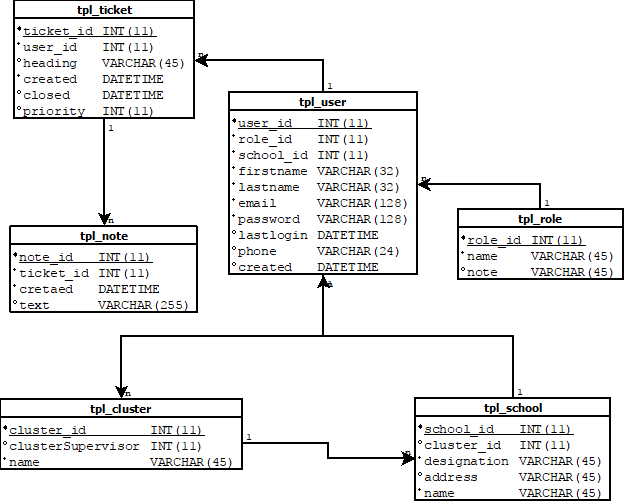
\includegraphics[scale=.7]{figures/JAVAeeDatabaseDiagramm.PNG}
	\caption{EER-Diagramm-Java-EE-Anwendung}
	\label{EER-Diagramm-Java-EE-Anwendung}
\end{figure}

\newpage

\subsubsection{tpl\_cluster}

In dieser Tabelle werden die Cluster festgelegt. Als Cluster wird eine Mengen von Schulen, die zu einer Organisation zusammen geschlossen wurden, bezeichnet. Jeder Cluster hat einen Supervisor, der für die Bearbeitung der anfallenden Tickets in ebendiesem Cluster verantwortlich ist.
Der Supervisor wird per Referenz zur User-Tabelle festgelegt. Ein Cluster hat immer genau einen Supervisor. Zusätzlich wird noch ein Name für den Cluster festgelegt.

\begin{table}[h]
	\begin{tabular}{|p{3.5cm}|p{4cm}|p{6.2cm}|}
		\hline
		\textbf{Column Name:} & \textbf{Datatype:} & \textbf{Content:}\\
		\hline
		cluster\_id & INT & Eindeutige ID des Clusters. Dieser Wert ist rein technisch und hat neben der Eindeutigkeit keine weitere Aussagekraft.\\
		\hline
		clusterSupervisor & INT & Referenz zu dem User der in diesem Cluster der Supervisor ist\\
		\hline
		name & VARCHAR(45) & Name des Clusters\\
		\hline
	\end{tabular}
	\caption{tab:tpl-cluster}
\end{table}
\label{tab:tpl_cluster}

\newpage

\subsubsection{tpl\_user}

In dieser Tabelle werden die User des Ticketsystems gehalten. Von jedem User werden der Vorname, Nachname, E-Mail-Adresse und das Passwort gespeichert. Optional kann auch der letzte Login, die Telefonnummer und das Datum, an dem der Account erstellt wurde, gespeichert werden.
Ein User muss einer Schule zugewiesen sein, um vollständig im System registriert zu werden. Ein User kann optional auch die Funktion des Supervisors eines Clusters einnehmen.
WICHTIG: lastlogin und created werden nach folgender Form in der Datenbank gespeichert "YYYY-MM-DD HH:MM:SS".

\begin{table}[h]
	\begin{tabular}{|p{3.5cm}|p{4cm}|p{6.2cm}|}
		\hline
		\textbf{Column Name:} & \textbf{Datatype:} & \textbf{Content:}\\
		\hline
		user\_id & INT & Eindeutige ID des User. Dieser Wert ist rein technisch und hat  neben der Eindeutigkeit keine weitere Aussagekraft.\\
		\hline
		role\_id & INT( & Referenz zu der Rolle die der User besitzt\\
		\hline
		school\_id & INT &  Referenz zu der Schule vom User \\
		\hline
		firstname & VARCHAR(32) & Vorname des Users\\
		\hline
		lastname & VARCHAR(32) & Nachname des Users\\
		\hline
		email & VARCHAR(128) & E-Mail-Adresse des Users\\
		\hline
		password & VARCHAR(128) & Das Passwort des Users in Hash Form \\
		\hline
		lastlogin & DATETIME & Das Datum, in oben angegebener Form, an dem sich der User zuletzt angemeldet hat \\
		\hline
		password & VARCHAR(24) & Das Passwort des Users in Hash Form \\
		\hline
		created & DATETIME & Das Datum, in oben angegebener Form, an dem der User angelegt worden ist\\
		\hline
	\end{tabular}
	\caption{tab:tpl-user}
\end{table}
\label{tab:tpl_user}

\newpage

\subsubsection{tpl\_ticket}

In dieser Tabelle werden die erstellten Tickets des Ticketsystems gespeichert. Das Ticket wird genau einem User zugeordnet und kann mehrere Notizen (notes) beinhalten. Des weiteren besteht ein Ticket aus einem Header, der Priorität und an welchem Datum das Ticket erstellt und geschlossen wurde.
WICHTIG: closed und created werden nach folgender Form in der Datenbank gespeichert "YYYY-MM-DD HH:MM:SS".

\begin{table}[h]
	\begin{tabular}{|p{3.5cm}|p{4cm}|p{6.2cm}|}
		\hline
		\textbf{Column Name:} & \textbf{Datatype:} & \textbf{Content:}\\
		\hline
		ticket\_id & INT & Eindeutige ID des Tickets. Dieser Wert ist rein technisch und hat neben der Eindeutigkeit keine weitere Aussagekraft.\\
		\hline
		user\_id & INT & Referenz zum User zu dem das Ticket gehört\\
		\hline
		heading & VARCHAR(45) &  Die Überschrift des Tickets\\
		\hline
		created & DATETIME & Das Datum, in oben angegebener Form, an dem das Ticket angelegt worden ist\\
		\hline
		closed & DATETIME & Das Datum, in oben angegebener Form, an dem das Ticket geschlossen worden ist\\
		\hline
		priority & INT & Hier wird die Priorität des Tickets angegeben. Kann eine Wert von 0-4 haben, der default Wert ist 0.\\
		\hline
	\end{tabular}
	\caption{tab:tpl-ticket}
\end{table}
\label{tab:tpl_ticket}

\newpage

\subsubsection{tpl\_note}

In dieser Tabelle werden die Notizen (notes) für die Tickets gespeichert. Jeder Notiz wird ein Ticket zugewiesen. Ein Ticket kann mehrere Notizen enthalten, umgekehrt aber gehört eine Notiz immer genau zu einem Ticket. Eine Notiz besteht aus einem Text und einem Datum, das angibt, wann die Notiz erzeugt worden ist.
WICHTIG: created wird in folgendem Format in der Datenbank gespeichert: "YYYY-MM-DD HH:MM:SS".

\begin{table}[h]
	\begin{tabular}{|p{3.5cm}|p{4cm}|p{6.2cm}|}
		\hline
		\textbf{Column Name:} & \textbf{Datatype:} & \textbf{Content:}\\
		\hline
		note\_id & INT & Eindeutige ID der Notiz. Dieser Wert ist rein technisch und hat neben der Eindeutigkeit keine weitere Aussagekraft.\\
		\hline
		ticket\_id & INT & Referenz zum Ticket dem diese Notiz angehört\\
		\hline
		created & DATETIME & Das Datum, in oben angegebener Form, an dem die Notiz angelegt worden ist\\
		\hline
		text & VARCHAR(255) & Ein Text der Informationen zum Ticket beinhaltet\\
		\hline
	\end{tabular}
	\caption{tab:tpl-note}
\end{table}
\label{tab:tpl_note}

\newpage

\subsubsection{tpl\_role}

In dieser Tabelle werden die Rollen gespeichert, die ein User annehmen kann. Eine Rolle besteht lediglich aus einem Namen und einer Notiz. Ein User kann genau eine Rolle haben, aber eine Rolle kann umgekehrt von mehreren Usern genutzt werden.

\begin{table}[h]
	\begin{tabular}{|p{3.5cm}|p{4cm}|p{6.2cm}|}
		\hline
		\textbf{Column Name:} & \textbf{Datatype:} & \textbf{Content:}\\
		\hline
		role\_id & INT & Eindeutige ID der Rolle. Dieser Wert ist rein technisch und hat neben der Eindeutigkeit keine weitere Aussagekraft.\\
		\hline
		name & VARCHAR(45) & Name der Rolle\\
		\hline
		note & VARCHAR(45) & Informationen über die Rolle\\
		\hline
	\end{tabular}
	\caption{tab:tpl-role}
\end{table}
\label{tab:tpl_role}


\subsubsection{tpl\_school}

In dieser Tabelle werden die Schulen gespeichert, die diese Ticketsystem verwenden.
Eine Schule wird mit ihrer Bezeichnung, Adresse und Namen abgespeichert. Des Weiteren kann eine Schule einem Cluster zugeordnet werden. 

\begin{table}[h]
	\begin{tabular}{|p{3.5cm}|p{4cm}|p{6.2cm}|}
		\hline
		\textbf{Column Name:} & \textbf{Datatype:} & \textbf{Content:}\\
		\hline
		school\_id & INT & Eindeutige ID der Schule. Dieser Wert ist rein technisch und hat neben der Eindeutigkeit keine weitere Aussagekraft.\\
		\hline
		cluster\_id & INT & Referenz zu dem Cluster dem die Schule angehört\\
		\hline
		designation & VARCHAR(45) & Schulbezeichnung der Schule\\
		\hline
		address & VARCHAR(45) & Die Adresse der Schule\\
		\hline
		name & VARCHAR(45) & Name der Schule\\
		\hline
	\end{tabular}
	\caption{tab:tpl-school}
\end{table}
\label{tab:tpl_school}

\newpage


\subsection{Beschreibung der Datenbankanbindung von unserem Java EE Prototyp}

Da unsere Anwendung nur ein Prototyp ist, wurde auch die Datenbankanbindung nur mit den wichtigsten Funktionen konzipiert. Deshalb ist die Klasse\\
\code{Datenbankanbindung.java} auch sehr statisch und redundant geschrieben. 
Die Datenbankanbindung wurde mit Hilfe der Java Api JDBC realisiert.\\
Mit Hilfe der get-Methoden lassen sich die einzelnen Tabellen aus der Datenbank auslesen und durch die insert-Methoden werden Einträge in die Tabelle eingefügt.
Mit der Methode \code{dbconnect} kann die Verbindung zu der Datenbank hergestellt werden.\\
\\
Am Anfang der Klasse werden drei String Variablen mit Informationen über den Datenbank-Zugang initialisiert.
\begin{itemize}
	\item \code{\$url:} Die URl unter der die Datenbank zu erreichen ist. In diesem Fall liegt die Datenbank Local auf einem Rechner, da es sich noch um einen Prototypen handelt.
	\item \code{\$username:} Ist ein User, der die benötigen Rechte hat, um lesend und schreibend auf die Datenbank zugreifen zu können. In unserem Fall greifen wir mit dem root User auf die Datenbank zu, da sie nur Local gespeichert ist und wir uns noch keine Gedanken über Sicherheit machen müssen.
	\item \code{\$password:} Ist das Passwort des User. 
\end{itemize}

\begin{lstlisting}[language=JAVA, caption=Datenbankanbindung.java/Datenfelder, firstnumber=30]
private String url = "jdbc:mysql://localhost:3306/java_ee_database";
private String username = "root";
private String password = "";
\end{lstlisting}
\newpage
Im folgenden werden die Methoden Klasse \code{Datenbankanbindung.java} im Detail beschrieben.
 
\subsubsection{Methode dbconnect\(\)}
Diese Methode stellt eine Verbindung zu der Datenbank her und liefert ein Statement Objekt zurück. Das Statement Objekt wird benötigt, um eine Query an die Datenbank zu schicken.
Um ein Statement Objekt erzeugen zu können, muss zuerst ein Connection Objekt erzeugt werden. Dies erfolgt durch die Methode \code{getConnection} mit den Parameter \code{url}, \code{username}, \code{password}. Konnte keine Verbindung zu der Datenbank hergestellt werden, wird durch den Catch-Block die \code{SQLException} gefangen und der Wert \code{null} zurück gegeben.

\begin{lstlisting}[language=JAVA, caption=Datenbankanbindung.java/Methode-dbconnect, firstnumber=44]
public Statement dbconnect()
{   
try
{
Connection connection = (Connection) DriverManager.getConnection(url, username, password);
Statement stmt = connection.createStatement();
return stmt;
}
catch(SQLException e)
{
return null;
}
}
\end{lstlisting}

\newpage

\subsubsection{Methode insertRole\(\)}

Bei dieser Methode wird ein Insert-Statement erzeugt und anschließend an die Datenbank geschickt, zurück bekommen wir den String 'Das Insert hat funktioniert.' oder \code{null}, wenn das Insert nicht funktioniert hat. Als Parameter werden die Values benötigt, welche man in die Datenbank schreiben möchte. Zuerst wird mit der Methode \code{dbconnect\(\)} ein Statment Objekt erstellt und darauffolgend wird mit Hilfe der \code{executeUpdate} Methode die Query an die Datenbank geschickt. Ist das Abschicken der Query nicht erfolgreich, bekommt man den Wert \code{null} zurück.\\
Dieser Methodenaufbau finden wir bei allen insert-Methoden dieser Klasse.

\begin{lstlisting}[language=JAVA, caption=Datenbankanbindung.java/Methode-dbconnect, firstnumber=271]
public String insertRole(String name, String note)
{
try
{
dbconnect().executeUpdate("INSERT INTO tpl_role 
(name, note) VALUES (\""+ name +"\", \""+ note +"\")");
return "Das Insert hat funktioniert";
}
catch(SQLException e)
{
return null;
}
}
\end{lstlisting}
\newpage
\subsubsection{Methode getRoles\(\)}

Mit Hilfe der Methode \code{getRoles} lassen sich alle Rollen aus der Datenbanktabelle \code{role} auslesen.
Zuerst wird in dieser Methode eine ArrayList \code{roles} initialisiert, anschließend werden String Variablen definiert, die benötigt werden, um aus dem \code{ResultSet} die Datenfelder der Rolle zu lesen.
Im try-Block wird nun ein SELECT-Statement an die Datenbank geschickt und ein \code{ResultSet} Objekt rs erzeugt. 
Um aus dem \code{ResultSet} die einzelnen Rollen auszulesen, benötigen wir eine while-Schleife. Diese iterieren solange durch das \code{ResultSet}, bis kein Eintrag mehr vorhanden ist\code{(bis rs.next() false zurück gibt)}.
In dieser while-Schleife wird zuerst ein \code{role} Objekt erzeugt und mit Hilfe der set-Methoden die Datenfelder dieses Rollenobjekts gesetzt. Zum Schluss wird das Rollenobjekt noch der ArrayList \code{roles} hinzugefügt. Wurde durch alle Einträge des \code{ResultSet} iteriert, wird das Statement geschlossen. Tritt während dem Durchlaufen des Try-Blockes ein Fehler auf, so wird der Wert \code{null} durch den Catch-Block zurückgegeben.\\ 
Diesen Methodenaufbau finden wir bei allen get-Methoden dieser Klasse.

\newpage


\begin{lstlisting}[language=JAVA, caption=Datenbankanbindung.java/Methode-getRoles, firstnumber=59]
public ArrayList getRoles()
{
ArrayList <tpl_role> roles = new ArrayList<>();

String value = "role_id";
String value1 = "name";
String value2 = "note";
try 
{
ResultSet rs = dbconnect().executeQuery("SELECT * FROM tpl_role");

while(rs.next())
{
tpl_role role = new tpl_role();
role.setName(rs.getString(value1));
role.setId(rs.getInt(value));
role.setNote(rs.getString(value2));
roles.add(role);
}
rs.close();
return roles;
} 
catch (SQLException ex) 
{
return null;
}
}
\end{lstlisting}

\renewcommand{\arraystretch}{1}

\newpage

%todo: ost ticket: User gendern? Betreuungslehrer fragen
%todo: null \code{null} wird so Formatiert + alle Klassen namen + Methodennamen
%todo: doppelpunkte bei aufzählung + \textbf durch \code ersetzen.
%todo: finales durchlesen der Doku
